\subsection{Vista}
\begin{figure}[!h]
	\centering
	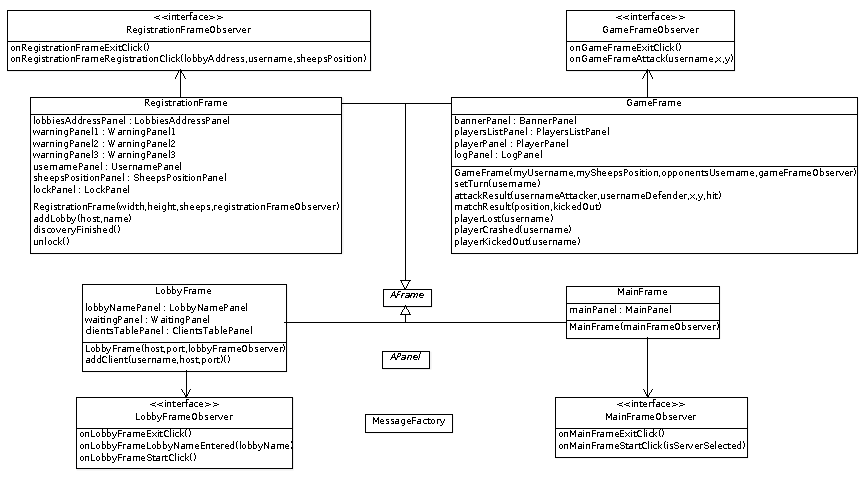
\includegraphics[scale=0.4, angle=90]{core/imgs/uml/vista}
	\caption{Diagramma delle Classi - Vista}
	\label{figure:class_diagram_view}
\end{figure}
Le classi della vista sono state implementate utilizzando la libreria
\textbf{Swing} fornita di default dal linguaggio.\newline
Come mostrato dal \textit{class diagram} in Figura
\ref{figure:class_diagram_view} i 4 frame del gioco estendono da un'unica
classe appositamente creata per fornire una veste grafica di default:
l'\textit{AFrame}. Questo è essenzialmente un JFrame con un layout grafico
prestabilito che fornisce metodi utili per l'aggiunta e la sostituzione dei
pannelli che sono di volta in volta visualizzati sui frame. È qui che viene
settato il nome del programma come titolo della finestra, l'icona del gioco e la
posizione di comparsa sul display (al centro).\newline
Così come per i frame, tutti i pannelli estendono da un'unica classe,
l'\textit{APanel}. Anch'esso fornisce metodi per l'aggiunta dei vari oggetti che
lo popoleranno (label, aree di testo, bottoni, ecc\dots). Ogni frame mantiene al
proprio interno le istanze dei pannelli da mostrare: in sequenza, come nel caso
della registrazione (prima il pannello che richiede la stanza alla quale
registrarsi, poi il pannello che richiede all'utente l'username, quello che
permette di inserire la posizione delle proprie pecore sul campo di gioco,
ecc\dots), o nelle varie parti, come nel caso del gioco (il pannello con il nome
del programma in alto, il pannello con i campi dei giocatori al centro, quello
con la lista di tutti i player a destra, ecc\dots).\newline
Un pattern molto importante e particolarmente sfruttato nell'implementazione
grafica di questo progetto è \textit{Observer}, il quale si basa su uno o più
oggetti (osservatori o observer) che vengono registrati e notificati
all'occorrenza di uno o più determinati eventi. Ogni pannello ha associato un
osservatore (un'interfaccia) che fornisce i metodi da implementare a qualunque
oggetto voglia essere notificato all'occorrenza di un evento. Così come ci sono
osservatori per i pannelli atti a notificare i frame quando accade qualcosa di
significativo, ogni frame ha a sua volta un osservatore associato che serve a
notificare le classi principali del gioco (Main, Lobby e Battlesheep)
all'occorrenza di determinati eventi scatenati dagli utenti. È in questo modo
che la grafica comunica con le classi sottostanti. Queste, a loro volta,
comunicano con le classi grafiche utilizzando direttamente i metodi che esse
espongono nella loro interfaccia.



\subsubsection{Main Frame}
\begin{figure}[!h]
	\centering
	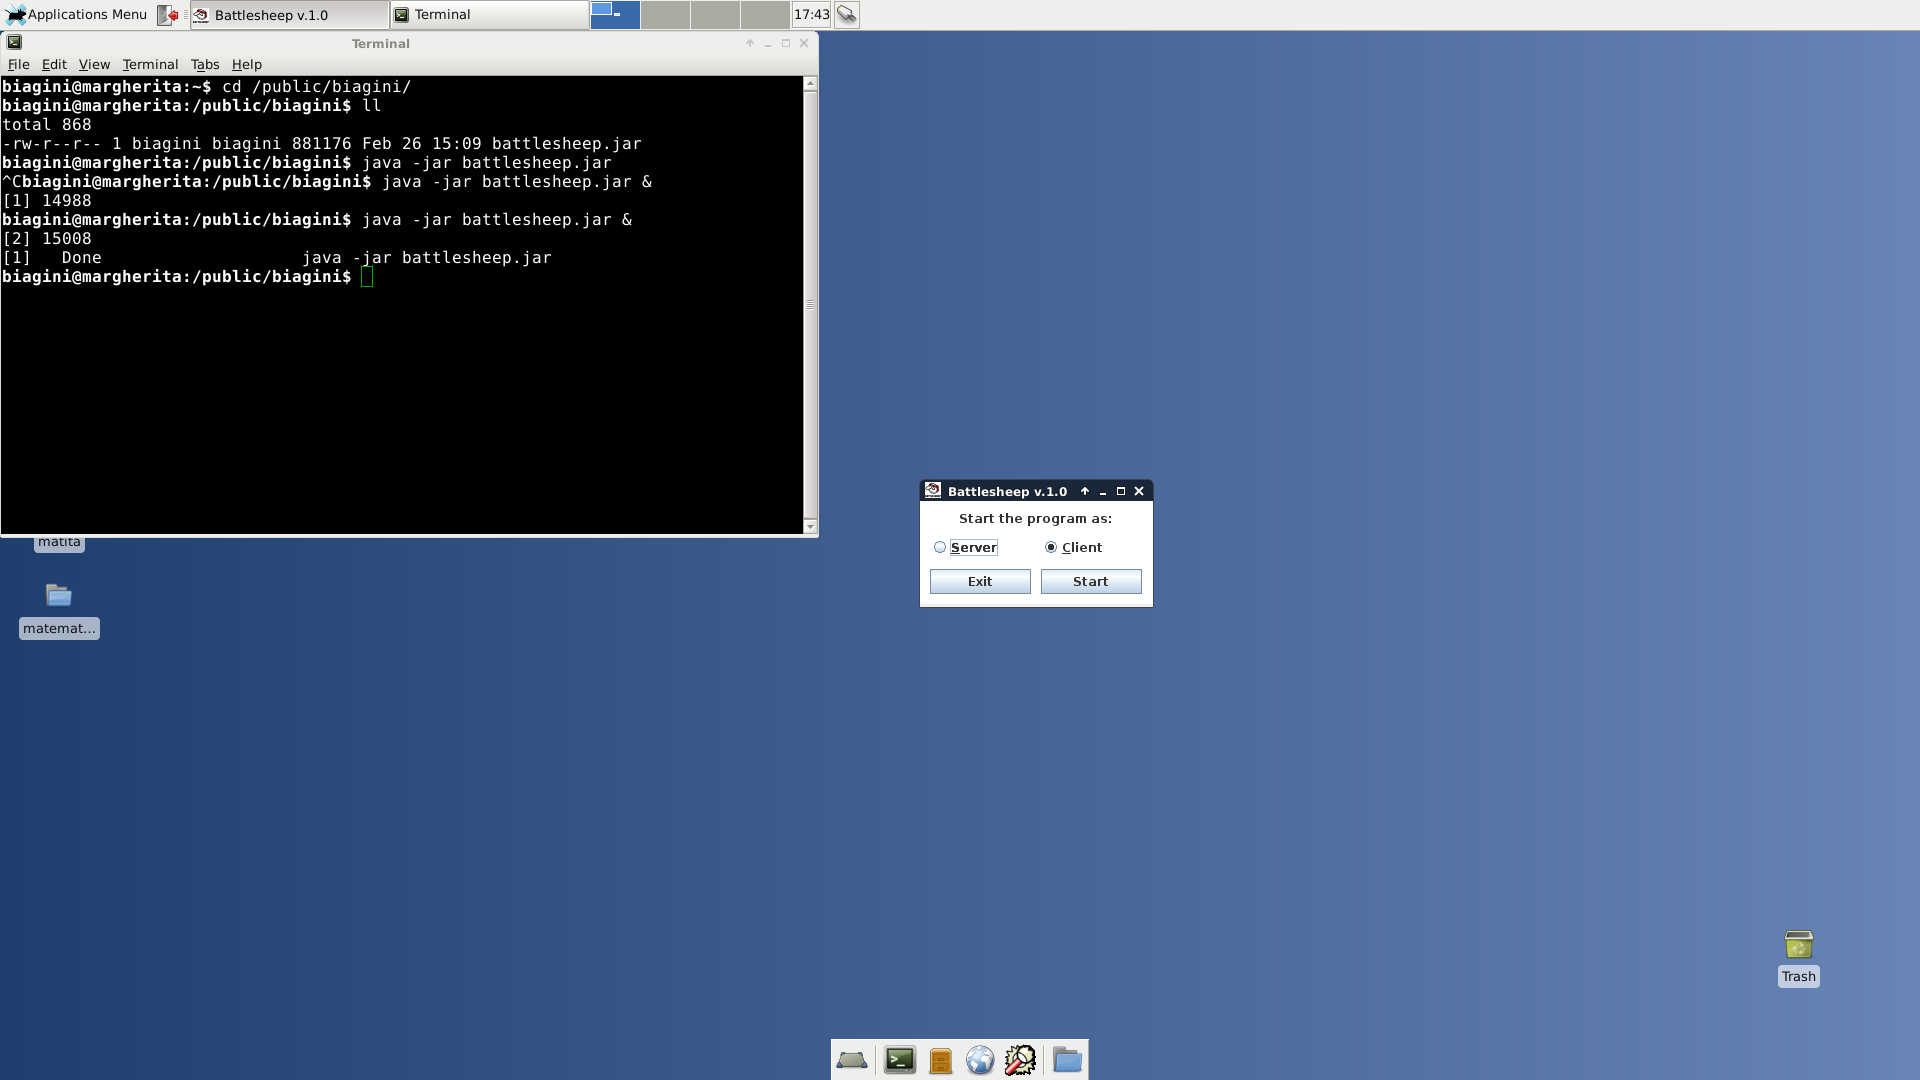
\includegraphics[scale=0.5]{core/imgs/gui/main_frame}
	\caption{Main Frame}
	\label{figure:main_frame}
\end{figure}
Il frame principale si compone di un unico pannello, il \textit{MainPanel},
mostrato in Figura~\ref{figure:main_frame}. Così come detto in fase di
progettazione (Sezione~\ref{subsubsection:progettazione_main_frame}), questo
frame ha il compito di permettere all'utente la scelta della modalità nella
quale avviare il programma: se come server (lobby) o come client (game).\newline
Il MainPanel, dunque, ha un osservatore associato che notifica il MainFrame alla
pressione dei bottoni ``exit'' e ``start'' il quale, a sua volta (tramite
l'observer \textit{MainFrameObserver}), notifica la classe Main dei medesimi
eventi passandole (nel caso in cui il bottone ``start'' sia premuto) la modalità
nella quale avviare il programma.



\subsubsection{Lobby Frame}
\begin{figure}
	\centering
	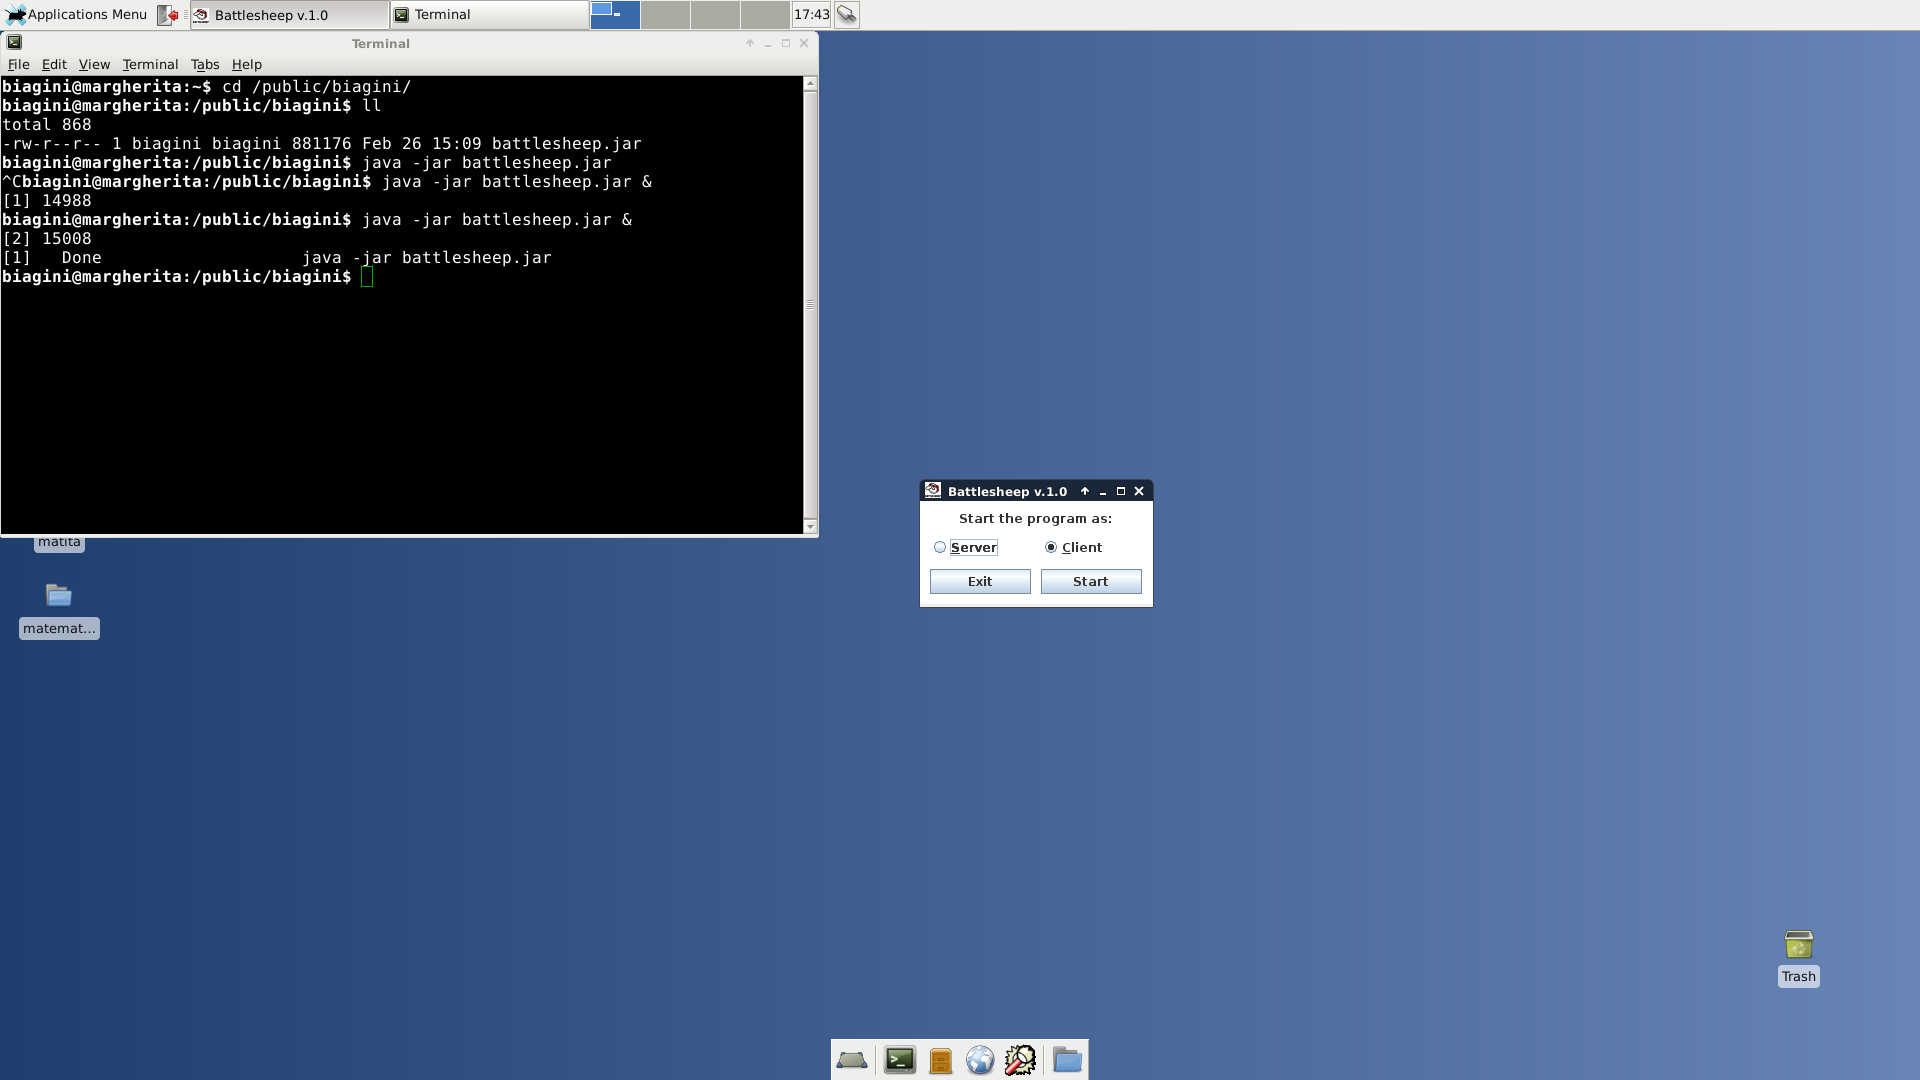
\includegraphics[scale=0.5]{core/imgs/gui/main_frame}
	\caption{Lobby Frame}
	\label{figure:lobby_frame}
\end{figure}

